%%%%%%%%%%%%%%%%%%%%%%%%%%%%%%%%%%%%%%%%%
% Wenneker Article
% LaTeX Template
% Version 2.0 (28/2/17)
%
% This template was downloaded from:
% http://www.LaTeXTemplates.com
%
% Authors:
% Vel (vel@LaTeXTemplates.com)
% Frits Wenneker
%
% License:
% CC BY-NC-SA 3.0 (http://creativecommons.org/licenses/by-nc-sa/3.0/)
%
%%%%%%%%%%%%%%%%%%%%%%%%%%%%%%%%%%%%%%%%%

%----------------------------------------------------------------------------------------
%	PACKAGES AND OTHER DOCUMENT CONFIGURATIONS
%----------------------------------------------------------------------------------------

\documentclass[10pt, a4paper, twocolumn]{article} % 10pt font size (11 and 12 also possible), A4 paper (letterpaper for US letter) and two column layout (remove for one column)

\usepackage[english]{babel} % English language hyphenation
\usepackage{microtype} % Better typography
\usepackage{amsmath,amsfonts,amsthm} % Math packages for equations
\usepackage[svgnames]{xcolor} % Enabling colors by their 'svgnames'
\usepackage[hang, small, labelfont=bf, up, textfont=it]{caption} % Custom captions under/above tables and figures
\usepackage{booktabs} % Horizontal rules in tables
\usepackage{lastpage} % Used to determine the number of pages in the document (for "Page X of Total")
\usepackage{graphicx} % Required for adding images
\usepackage{amssymb}
\usepackage[table]{xcolor}
\usepackage{enumitem} % Required for customising lists
\setlist{noitemsep} % Remove spacing between bullet/numbered list elements
\usepackage{sectsty} % Enables custom section titles
\allsectionsfont{\usefont{OT1}{phv}{b}{n}} % Change the font of all section commands (Helvetica)
\usepackage{hyperref}
\usepackage[sort,numbers]{natbib}
%----------------------------------------------------------------------------------------
%	MARGINS AND SPACING
%----------------------------------------------------------------------------------------
\usepackage{geometry} % Required for adjusting page dimensions
\geometry{
	top=0.65cm, % Top margin
	bottom=1.5cm, % Bottom margin
	left=1.5cm, % Left margin
	right=1.5cm, % Right margin
	includehead, % Include space for a header
	includefoot, % Include space for a footer
	%showframe, % Uncomment to show how the type block is set on the page
}
\setlength{\columnsep}{6mm} % Column separation width


%----------------------------------------------------------------------------------------
%	FONTS
%----------------------------------------------------------------------------------------

\usepackage[T1]{fontenc} % Output font encoding for international characters
\usepackage[utf8]{inputenc} % Required for inputting international characters

\usepackage{XCharter} % Use the XCharter font



%\input{structure.tex} % Specifies the document structure and loads requires packages

%----------------------------------------------------------------------------------------
%	ARTICLE INFORMATION
%----------------------------------------------------------------------------------------

\title{Robhoot \\ Knowledge Open Network} % The article title
  \author{XX{\textsuperscript{1,2,3} and XY\textsuperscript{2,3}} % Authors
  \newline\newline % Space before institutions
  \\
	\textsuperscript{1}\institution{}\\ % Institution 1
	\textsuperscript{2}\institution{}\\ % Institution 2
	%\textsuperscript{3}\institution{\texttt{LaTeXTemplates.com}}
      %} % Institution 3


% Example of a one line author/institution relationship
%\author{\newauthor{John Marston} \newinstitution{Universidad Nacional Autónoma de México, Mexico City, Mexico}}

\date{\today} % Add a date here if you would like one to appear underneath the title block, use \today for the current date, leave empty for no date
%---------------------------------------------------------------------------------------

\begin{document}

\maketitle % Print the title
\thispagestyle{firstpage} % Apply the page style for the first page (no headers and footers)

%----------------------------------------------------------------------------------------
%	ABSTRACT
%----------------------------------------------------------------------------------------
\lettrineabstract{\section{{\bf Summary}} The Robhoot project aims to
  connect open-access research and the public in a decentralized
  network to help taking informed decisions when solving complex
  social, environmental and technological problems. Current
  technologies for scientific inquiry and decision-making are highly
  fragmented and thus only increase robustness, reproducibility,
  open-access and the interactions with the public marginally. The
  goal of Robhoot is to propose a hybrid-neutral-technology to lay out
  the foundation for an open-science research ecosystem aiming to
  strengthen the robustness and reproducibility of science by fully
  automating standard reporting in decision-making. Robhoot is not set
  out to deliver a finished deep knowledge network in the science
  ecosystem, but to provide a science-enabled technology in
  establishing a prototype proof-of-principle to connect decentralized
  and neutral-knowledge generation with knowledge-inspired societies.}
%----------------------------------------------------------------------------------------
%	ARTICLE CONTENTS
%----------------------------------------------------------------------------------------
\section{The Science Ecosystem}
The process of building science and technology requires multiple steps
of information transfer among trusted/untrusted peers to build solid
evidence-based knowledge. Evidence-based knowledge forms the basis of
decisions across all human activities. In this regard, reliable,
open-access, neutral, and immutable evidence-based knowledge following
a secure peer-to-peer architecture storing the open-source knowledge
graphs derived from distributed research outputs is far from
reality. For example, reproducibility, decentralization, and
immutability of knowledge is key to have fully neutral open-access
reports when taking informed decisions in complex societal,
environmental and technological problems. However, currently public
funded science is highly centralized \citep{Inhaber1977,Gunter2018}⁠⁠,
prone to errors \citep{Fang2011}, difficult to reproduce
\citep{Hardwicke2018}, and contains many biases
\citep{Ioannidis2005}. Actually, these elements make the connection
between the scientific process, open-access and reproducible reporting
for decision-making highly improbable. Despite many projects are
aiming at making the science ecosystem less centralized and biased
while increasing openness and reproducibility a science-enabled
technological paradigm connecting open-science to knowledge-inspired
societies is not currently in place \citep{Gunther2018}.

Many studies in decentralized ecosystems are producing an immense gain
in detailed knowledge about scalability, security and decentralization
trade-offs
\citep{Golem2016,Durov2017,Androulaki2018,OceanProtocolFoundation2018,BigchainDBGmbH2018}. Automation
and AI technologies is the other angle from which many advances are
rapidly occurring \citep{Schmidhuber:2015,Reichstein,Gil2019}. Yet,
while the existing technological paradigm is rapidly shifting towards
science-based decentralization and automation technologies, end-to-end
open-source research accounting for decentralized, neutral and
automated knowledge-inspired technologies are missing. Rapid advances
of automated research platforms facilitating data integration
accounting for sections of the research cycle are currently under
development\footnote{This is by no means an exhaustive list but it
  gives an indication of the many projects currently in place:
  \href{https://www.nterminal.com}{NakamotoT},\href{https://cloud.google.com/bigquery/}{BigQuery},\href{https://www.automaticstatistician.com/index/}{Automated
    statistician},\href{http://www.modulos.ai/}{Modulos},\href{https://ai.google/}{Google
    AI},\href{https://iris.ai}{Iris},\href{https://github.com/DS3Lab/easeml}{easeml}}
but open-source decentralized automated platforms accounting for the
research cycle are still at a very incipient stage of
development. While conceptual frameworks conceptualizing the required
layers in many research fields are well established (Figure 1a), there
is currently a lack of integration and development of tools connecting
knowledge graphs (Figure 1b) into deep process-based learning networks
to explore their robustness (Figure 1c) in fully decentralized
ecosystems (Figure 1d).

\begin{table}
 %\rowcolor{pink}
\begin{tabular}{ p{3cm} | p{2cm} | p{2cm}}
  \hline \hline
  \textbf{Features} & \textbf{Science Ecosystem} &\textbf{Robhoot 1.0}\\  \hline
  Decentralization & No & Yes \\ \hline
  Open-access & Mostly No & Yes \\ \hline
  Immutability & No & Yes \\ \hline
  Robustness & Mostly No & Yes \\ \hline
  Reproducibility & Mostly No & Yes \\ \hline        
  Owner-Controlled assets & No & Yes \\ \hline       
  \bottomrule

\end{tabular}
\caption{Robhoot aims to be designed to resolve desirable properties
  of science: Robustness, Reproducibility, Decentralization, Open and
  Direct access to reporting by peers and not-peers.}
\end{table}
% ------------------------------------------------
  \section{Robhoot Design Goals}
  Robhoot aims to build an automated knowledge network technology to
  connect knowledge-graphs to knowledge-inspired societies (Figure
  1). Robhoot will be built on different stages following standard
  version protocols. The most advanced version is to provide real-time
  open-access and decentralized neutral data-rule-knowledge to gain
  informed decisions when solving complex social, environmental and
  technological problems. Figures 1 and 2 show Robhoot stages and the
  timeline of each stage, respectively.
  \includegraphics[width=0.45\textwidth]{Figure1.pdf}
  
  {\small {\bf Figure 1: Automated knowledge-based network
      technology}. {\bf a}) {\bf Robhoot 1.0} aims to account for a
    end-to-end research cycle from data integration (top) to reporting
    generation (bottom). {\bf b}) {\bf Robhoot 2.0} will integrate a
    end-to-end research cycle with a knowledge graph (KG) represented
    as one research path of {\bf a} (i.e., Renku open-source
    code). {\bf c}) {\bf Robhoot 3.0} will account for deep
    knowledge-based networks to automatically explore populations of
    KGs to gain robustness of the process-based patterns contained in
    the data. {\bf d}) {\bf Robhoot 4.0} will deploy all KGs in a
    distributed network of mutually trusting/untrusting peers with
    every peer maintaining the population of the KGs (i.e.,
    decentralized P2P git network like Gitchain.)}
  
  The overall objectives for each of the four major Robhoot versions are the following:
  \vspace{-0.15 in}
   \subsection{Robhoot 1.0: Automated end-to-end Research Cycle}
   \begin{itemize}
   \item Develop, deploy and integrate open-source algorithms to
     automate an end-to-end research cycle (Figure 1a).
   \item Robustness within and between layers from data integration,
     complexity reduction, inference, and validation to visualization
     and automated reporting (Figure 1a).
   \item Robhoot 1.0 Open Network in Biodiversity and Global Change Research to connect
   open science (i.e., citizen and other models) to real-time open-access data-rule-knowledge
   to gain informed decisions when solving local and global
   environmental problems.
 \end{itemize}
 \vspace{-0.15 in}
 
  \subsection{Robhoot 2.0: Knowledge Graphs}
  \begin{itemize}
  \item Integration between the automated end-to-end research cycle with Knowledge Graphs (KGs) (Figure 1b).
  \item Robustness and stability of a suite of open-source lineage client-tracker algorithms.
  \end{itemize}
  \vspace{-0.15 in}
  
  \subsection{Robhoot 3.0: Deep learning networks}
  \begin{itemize}
  \item Deploy automated deep learning algorithms accounting for a
    end-to-end research cycle in a lineage client-tracker to produce
    populations of Knowledge Graphs (KGs) (Figures 1a-c).
  \item Robustness of the multi-objective optimization by exploring a
    suite of neural networks algorithms with lineage client-tracker
    paths in the multilayer network (Figure 1c).
  \end{itemize}
  \vspace{-0.15 in}
  
  \subsection{Robhoot 4.0: Distributed ledger network}
  \begin{itemize}
  \item Deploy an end-to-end permissioned-permissionless distributed
    ledger technology to guarantee decentralization, open-access and
    security of the KGs populations in the science ecosystem (Figures
    1c and 1d.)
  \item Distributed ledger implementation accounting for consensus
    algorithms and smart contracts among trusted-untrusted
    peer-to-peer interactions (Figure 1d).
  \item Exploring consensus algorithms to minimize
    scalability-security-decentralization trade-offs when storing the
    KGs in the knowledge network (Figure 1d).
  \item Testnet for the interaction between consensus protocols and
    the scalability-security-decentralization trade-offs when
    committing the KGs to the distributed ledger.
  \item Mainnet to cryptographically link each population of KGs to
    previous KGs-ledger to create an historical KGs-ledger chain that
    goes back to the genesis ledger. The mainnet aims to connect
    database real-time open-access citizen data science to
    knowledge-inspired societies.
  \end{itemize}
  
  \section{The multilayer nature of Robhoot}
  The science ecosystem currently lack technologies automating the
  full research cycle from end-to-end and its connection to the
  scalability-security-decentralization trade-offs of digital
  ecosystems. Despite, public institutions are demanding more
  reproducibility and openness of the data and the scientific process,
  and overall a shifting towards open and reproducible scientific and
  engineering landscapes, there are not currently open and integrated
  technologies aiming to compactly facilitate and distribute the
  scientific and engineering knowledge in reproducible and immutable
  knowledge networks.
  
  Knowledge generation usually comes from interactions within- and
  between-layers (Figure 1a). The feedbacks occurring among layers in
  the science and technology ecosystem also provide unexpected
  behaviors that are difficult to anticipate. Therefore many feedbacks
  and interactions within- and between-layers are not easy to
  reproduce if not properly accounted for. Robhoot will take advantage
  of the multilayer networks framework to explore how knowledge graphs
  and peer-to-peer interactions might connect to the robustness and
  reproducibility of the scientific process. The following are the six
  components required to complete Robhoot 1.0:

  \subsection{Data integration}
  Despite open-source ETLs are rapidly evolving towards accounting for
  many aspects of data integration (formats, historical-real time,
  storage, dimensions, size, bias and spatiotemporal resolution),
  there is a missing component in quantifying the robustness of
  knowledge that integrated data can provide. Automated populations of
  KGs connecting cutting-edge open-source ETLs to inference
  classification schemes can provide the quantification of robustness
  in knowledge-based patters for future predictive technologies.
  \subsection{Complexity reduction}

  \subsection{Inference}
  The integration between open-source data integration and inference
  schemes, the interlayer automation (O1: Multilayer), will allow for
  the systematic exploration of robust knowledge-based patterns when
  exploring the population of KGs. This is in sharp contrast to
  existing AI technologies mostly oriented to prediction without
  knowledge-based understanding. 

  \subsection{Validation}

  \subsection{Visualization}

  \subsection{Reporting}

  
  \section{Robhoot in Digital Ecosystems}
  Technologies with the capacity to compactly account for neutral,
  borderless, immutable, and open-access information in hybrid,
  trusted-untrusted peer-to-peer interactions, accounting for the
  multilayer nature of science and engineering are currently not in
  place. Producing such technologies will require interactions with
  the existing and rapidly evolving digital ecosystem in addition to
  integrating expertise from disparate disciplines like multilayer
  networks, deep learning, automation algorithmics, and distributed
  technologies. The integration of these disciplines will require to
  go beyond domain boundaries. Specifically, we will merge scientists
  and engineers from data and computer science, the physics of complex
  systems, artificial intelligence and the biology, ecology and
  evolution of social, natural and technological ecosystems to develop
  a hybrid technology: automated knowledge generation in a neutral,
  borderless and immutable network synthesized anew from existing
  open-source projects like Renku, Fabric and gitchain. The following
  are the three main domains from where Robhoot will benefit the most:
\subsection{Computing Power}
\subsection{Decentralization}
\subsection{Neural Networks}

\section{How to contribute to Robhoot}

\newpage
\section{The Robhoot roadmap}


\begin{figure*}[ht]
  \centering \includegraphics[width=1\textwidth]{GanttChart.pdf}
  {\small {\bf Figure 2: The Robhoot roadmap}: {\bf a}) {\bf Robhoot
      1.0} contains four working packages .... {\bf b}) {\bf Robhoot
      2.0} contains three packages to integrate a end-to-end research
    cycle with a knowledge graph (KG). {\bf c}) {\bf Robhoot 3.0}
    contains four packages ... deep knowledge-based networks to
    automatically explore populations of KGs to gain robustness of the
    process-based patterns contained in the data. {\bf d}) {\bf
      Robhoot 4.0} contains two packages to deploy all KGs in a
    distributed network of mutually trusting/untrusting peers with
    every peer maintaining the population of the KGs (i.e.,
    decentralized P2P git network like Gitchain.)}
\end{figure*}


\newpage
\section{Conclusion}
Science and technology ecosystems are in need of accounting for the
uncertainties, the reproducibility and the immutability related to
automation. This need is not just for a specific stage of the research
cycle, but for the full research cycle, from data acquisition to
automated reporting generation because knowledge-inspired societies
and governance will demand full research cycle transparency to solve
complex social, environmental and technological problems. This need
brings many challenges to our research proposal because obtaining
robust knowledge from integrating many layers of the research cycle,
each containing its own set of methods and uncertainties, can generate
divergent, fragile and contradictory outcomes.

We will develop a flexible research method focusing step by step in
different levels of complexity (i.e., from Robhoot 1.0 to 4.0). Our
motivation will be to provide a first open-access proof of concept of
how the technology works: we will automate reproducible research paths
along a multilayer network (Robhoot 1.0) to sample the KGs (Robhoot
2.0) using different deep learning algorithms to estimate the
uncertainty of the ruled-based inference obtained by fitting
predictions to simulated data (Robhoot 3.0). Accounting for the
uncertainties of each of the research stages when sampling the KGs
comes from the many distinct paths within and across the layers in the
research cycle (Figure 1). We will test a variety of consensus
algorithms to explore the degree of security, decentralization and
scalability of the ledger knowledge network using the generated
population of KGs (Robhoot 4.0).

Despite our focus will be bias towards the algorithmic robustness
during the four stages of Robhoot development, we will develop a
domain-specific case study, a Robhoot Open Network, to test the
robustness of the rule-based inference obtained by fitting each of the
generated KG to empirical patterns. The high risk associated to
robustly automate the full research cycle for producing immutable open
knowledge will be buffered to a great extend because the existing
digital ecosystem of tested and reliable open-source tools: We will
combine our own algorithms (i.e., add-hoc data integration algorithms
and neural-biological networks for deep learning algorithms for
sampling and automating the KGs) with open-source tools part of a
rapidly evolving open-digital ecosystem.

%----------------------------------------------------------------------------------------
%	BIBLIOGRAPHY
%----------------------------------------------------------------------------------------

%\printbibliography[title={Bibliography}] % Print the bibliography, section title in curly brackets

\newpage
\bibliographystyle{unsrtnat}
%\bibliographystyle{tree.bst}
\bibliography{Robhoot.bib}

%----------------------------------------------------------------------------------------

\end{document}

\hspace{-0.2 in}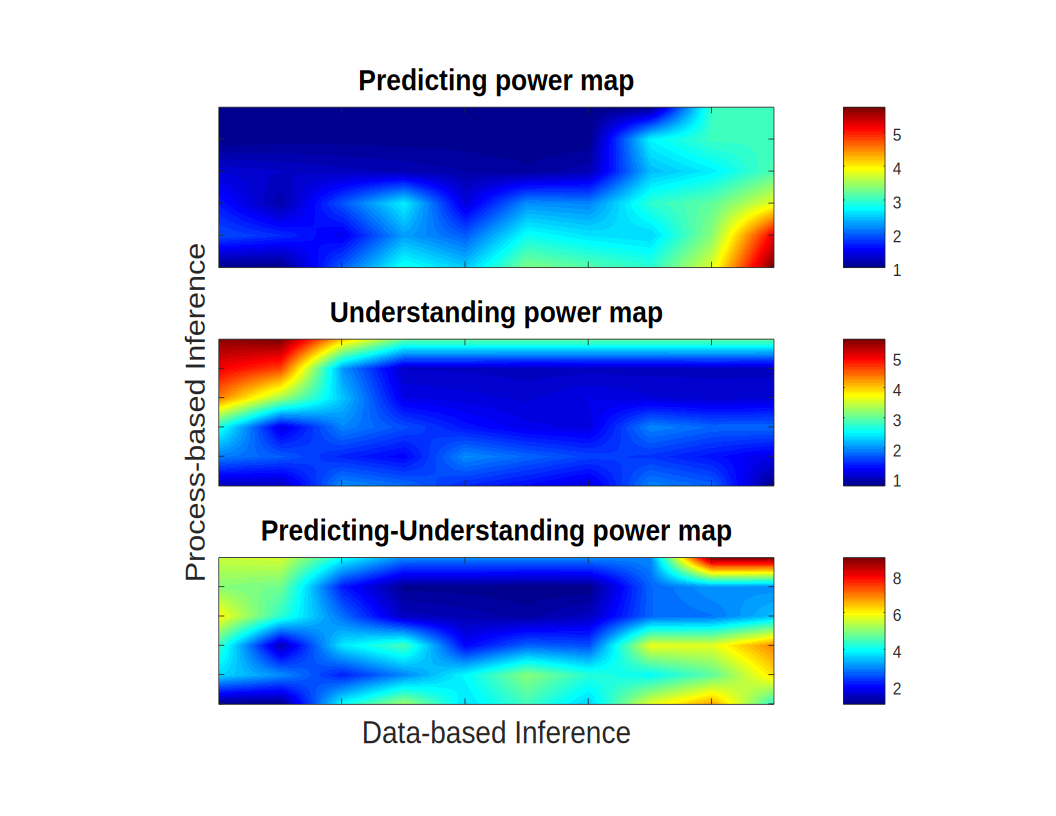
\includegraphics[width=0.52\textwidth]{Figure3.pdf}
{\small {\bf Figure 1: Prediction power (top), understanding (middle),
    and prediction-understanding power maps (bottom)}. x-axis
  represents data-based inference (i.e., gradient of AI methods from
  low (left) to high (right) predictive power). y-axis represents
  process-based inference (i.e., gradient of process-based methods
  from low (bottom left) to high (top left) understanding power). The
  gradient of predicting power map (top) shows a hot spot red area in
  the bottom right highlighting the region where AI methods best
  predict the empirical data. The gradient of understanding power map
  (middle) shows a red hot spot in the top left highlighting the
  region where the best mechanistic understanding occur. The
  predicting-understanding power map (bottom) shows the sum of the two
  previous maps highlighting a red hot spot where the best synthesis
  research joining predicting and understanding power of the empirical
  data might occur. The first research goal of this proposal aims to
  build an automated research platform to maximize the predicting and
  understanding power highlighted in the red hot spot of the
  predicting-understanding power map (bottom).}
